\documentclass[final]{beamer}\usepackage[]{graphicx}\usepackage[]{color}
%% maxwidth is the original width if it is less than linewidth
%% otherwise use linewidth (to make sure the graphics do not exceed the margin)
\makeatletter
\def\maxwidth{ %
  \ifdim\Gin@nat@width>\linewidth
    \linewidth
  \else
    \Gin@nat@width
  \fi
}
\makeatother

\definecolor{fgcolor}{rgb}{0.345, 0.345, 0.345}
\newcommand{\hlnum}[1]{\textcolor[rgb]{0.686,0.059,0.569}{#1}}%
\newcommand{\hlstr}[1]{\textcolor[rgb]{0.192,0.494,0.8}{#1}}%
\newcommand{\hlcom}[1]{\textcolor[rgb]{0.678,0.584,0.686}{\textit{#1}}}%
\newcommand{\hlopt}[1]{\textcolor[rgb]{0,0,0}{#1}}%
\newcommand{\hlstd}[1]{\textcolor[rgb]{0.345,0.345,0.345}{#1}}%
\newcommand{\hlkwa}[1]{\textcolor[rgb]{0.161,0.373,0.58}{\textbf{#1}}}%
\newcommand{\hlkwb}[1]{\textcolor[rgb]{0.69,0.353,0.396}{#1}}%
\newcommand{\hlkwc}[1]{\textcolor[rgb]{0.333,0.667,0.333}{#1}}%
\newcommand{\hlkwd}[1]{\textcolor[rgb]{0.737,0.353,0.396}{\textbf{#1}}}%

\usepackage{framed}
\makeatletter
\newenvironment{kframe}{%
 \def\at@end@of@kframe{}%
 \ifinner\ifhmode%
  \def\at@end@of@kframe{\end{minipage}}%
  \begin{minipage}{\columnwidth}%
 \fi\fi%
 \def\FrameCommand##1{\hskip\@totalleftmargin \hskip-\fboxsep
 \colorbox{shadecolor}{##1}\hskip-\fboxsep
     % There is no \\@totalrightmargin, so:
     \hskip-\linewidth \hskip-\@totalleftmargin \hskip\columnwidth}%
 \MakeFramed {\advance\hsize-\width
   \@totalleftmargin\z@ \linewidth\hsize
   \@setminipage}}%
 {\par\unskip\endMakeFramed%
 \at@end@of@kframe}
\makeatother

\definecolor{shadecolor}{rgb}{.97, .97, .97}
\definecolor{messagecolor}{rgb}{0, 0, 0}
\definecolor{warningcolor}{rgb}{1, 0, 1}
\definecolor{errorcolor}{rgb}{1, 0, 0}
\newenvironment{knitrout}{}{} % an empty environment to be redefined in TeX

\usepackage{alltt}
\usepackage[orientation = landscape, size = a0, scale = 1.4]{beamerposter}

\usepackage{amsmath, amsthm}
\usepackage[]{graphicx}
\usepackage{parskip, microtype}
\usepackage{caption, subcaption, multirow}
\usepackage{morefloats, hyperref}
\usepackage{rotating, longtable}
\usepackage[sort&compress, numbers]{natbib}

\usetheme{confposter}


\newlength{\sepwid}
\newlength{\onecolwid}
\newlength{\twocolwid}
\newlength{\threecolwid}
\setlength{\paperwidth}{48in} % A0 width: 46.8in
\setlength{\paperheight}{36in} % A0 height: 33.1in
\setlength{\sepwid}{0.024\paperwidth} % Separation width (white space) between columns
\setlength{\onecolwid}{0.22\paperwidth} % Width of one column
\setlength{\twocolwid}{0.464\paperwidth} % Width of two columns
\setlength{\threecolwid}{0.708\paperwidth} % Width of three columns

\def\newblock{\hskip .11em plus .33em minus .07em}





\title{Cosmopolitan and endemism dynamics of terrestrial mammals across the Cenozoic}
\author{Peter D Smits}
\institute{Committee on Evolutionary Biology, University of Chicago}
\IfFileExists{upquote.sty}{\usepackage{upquote}}{}

\begin{document}
\begin{frame}[t]
  \begin{columns}
    \begin{column}{\onecolwid}
      \begin{block}{}
        \begin{abstract}
          %This is where the abstract would go.
          How life history traits, such as diet, are related to the distribution of taxa across the landscape.
        \end{abstract}
        
      \end{block}
      \begin{block}{Introduction}
% trophic structure change through time
%   constituent taxa
%   paleo record
%     sampling (lack of abundance in terrestrial systems)
%     site occupancy/distribution
%   evolution of community
%     Damuth1982 on preservation of structure
%     Roopnarine2010,Roopnarine2012b,Roopnarine2007,
%     Roopnarine2006,Mitchell2012,Angielczyk2005
%
% distribution of organisms across the landscape
% how does life history affect distribution?
% how does taxonomic distribution change over time
%   life history characters
%     diet
%     life habit/locomotor category
%   abiotic factors
%     climate Zachos2001,Zachos2008
%
% previous work on contribution of different taxa to site similarity
%   Jernvall2004
%   Jernvall2002
%
  
        Previous work on mammalian site similarity has focused on organismal dietary distributions of terrestrial mammals in the Neogene Old World \citep{Jernvall2002,Jernvall2004}. 
        Here, I expand that analysis the entire Cenozoic of North America and analyze both diety and locomotor categories of terrestrial mammals.
      \end{block}

      \begin{block}{Methods}
        Mammalian taxonomic occurence information was obtained from the Paleobiology Database (\url{http://www.paleodb.org}).
        Taxonomic occurence information was restricted to only mammals occuring in North America during the Cenozoic.
        Ambiguously identified taxa were excluded from all analyses (e.g. aff., cf., ?).
        Temporal, geologic, dietary and life habit informaiton was also compiled for all taxa.

        Because terrestrial assemblages across the Cenozoic do not preserve as complete a record of community structure, taxonomic abundance distributions were not analyzed.

        %Temporal bins: stage, 2My

        %biogeographic networks
        Following \citet{Sidor2013} and \citet{Vilhena2013}

      \end{block}

      \begin{block}{Relative abundance}
        %\begin{figure}[ht]
        %  \begin{center}
        %    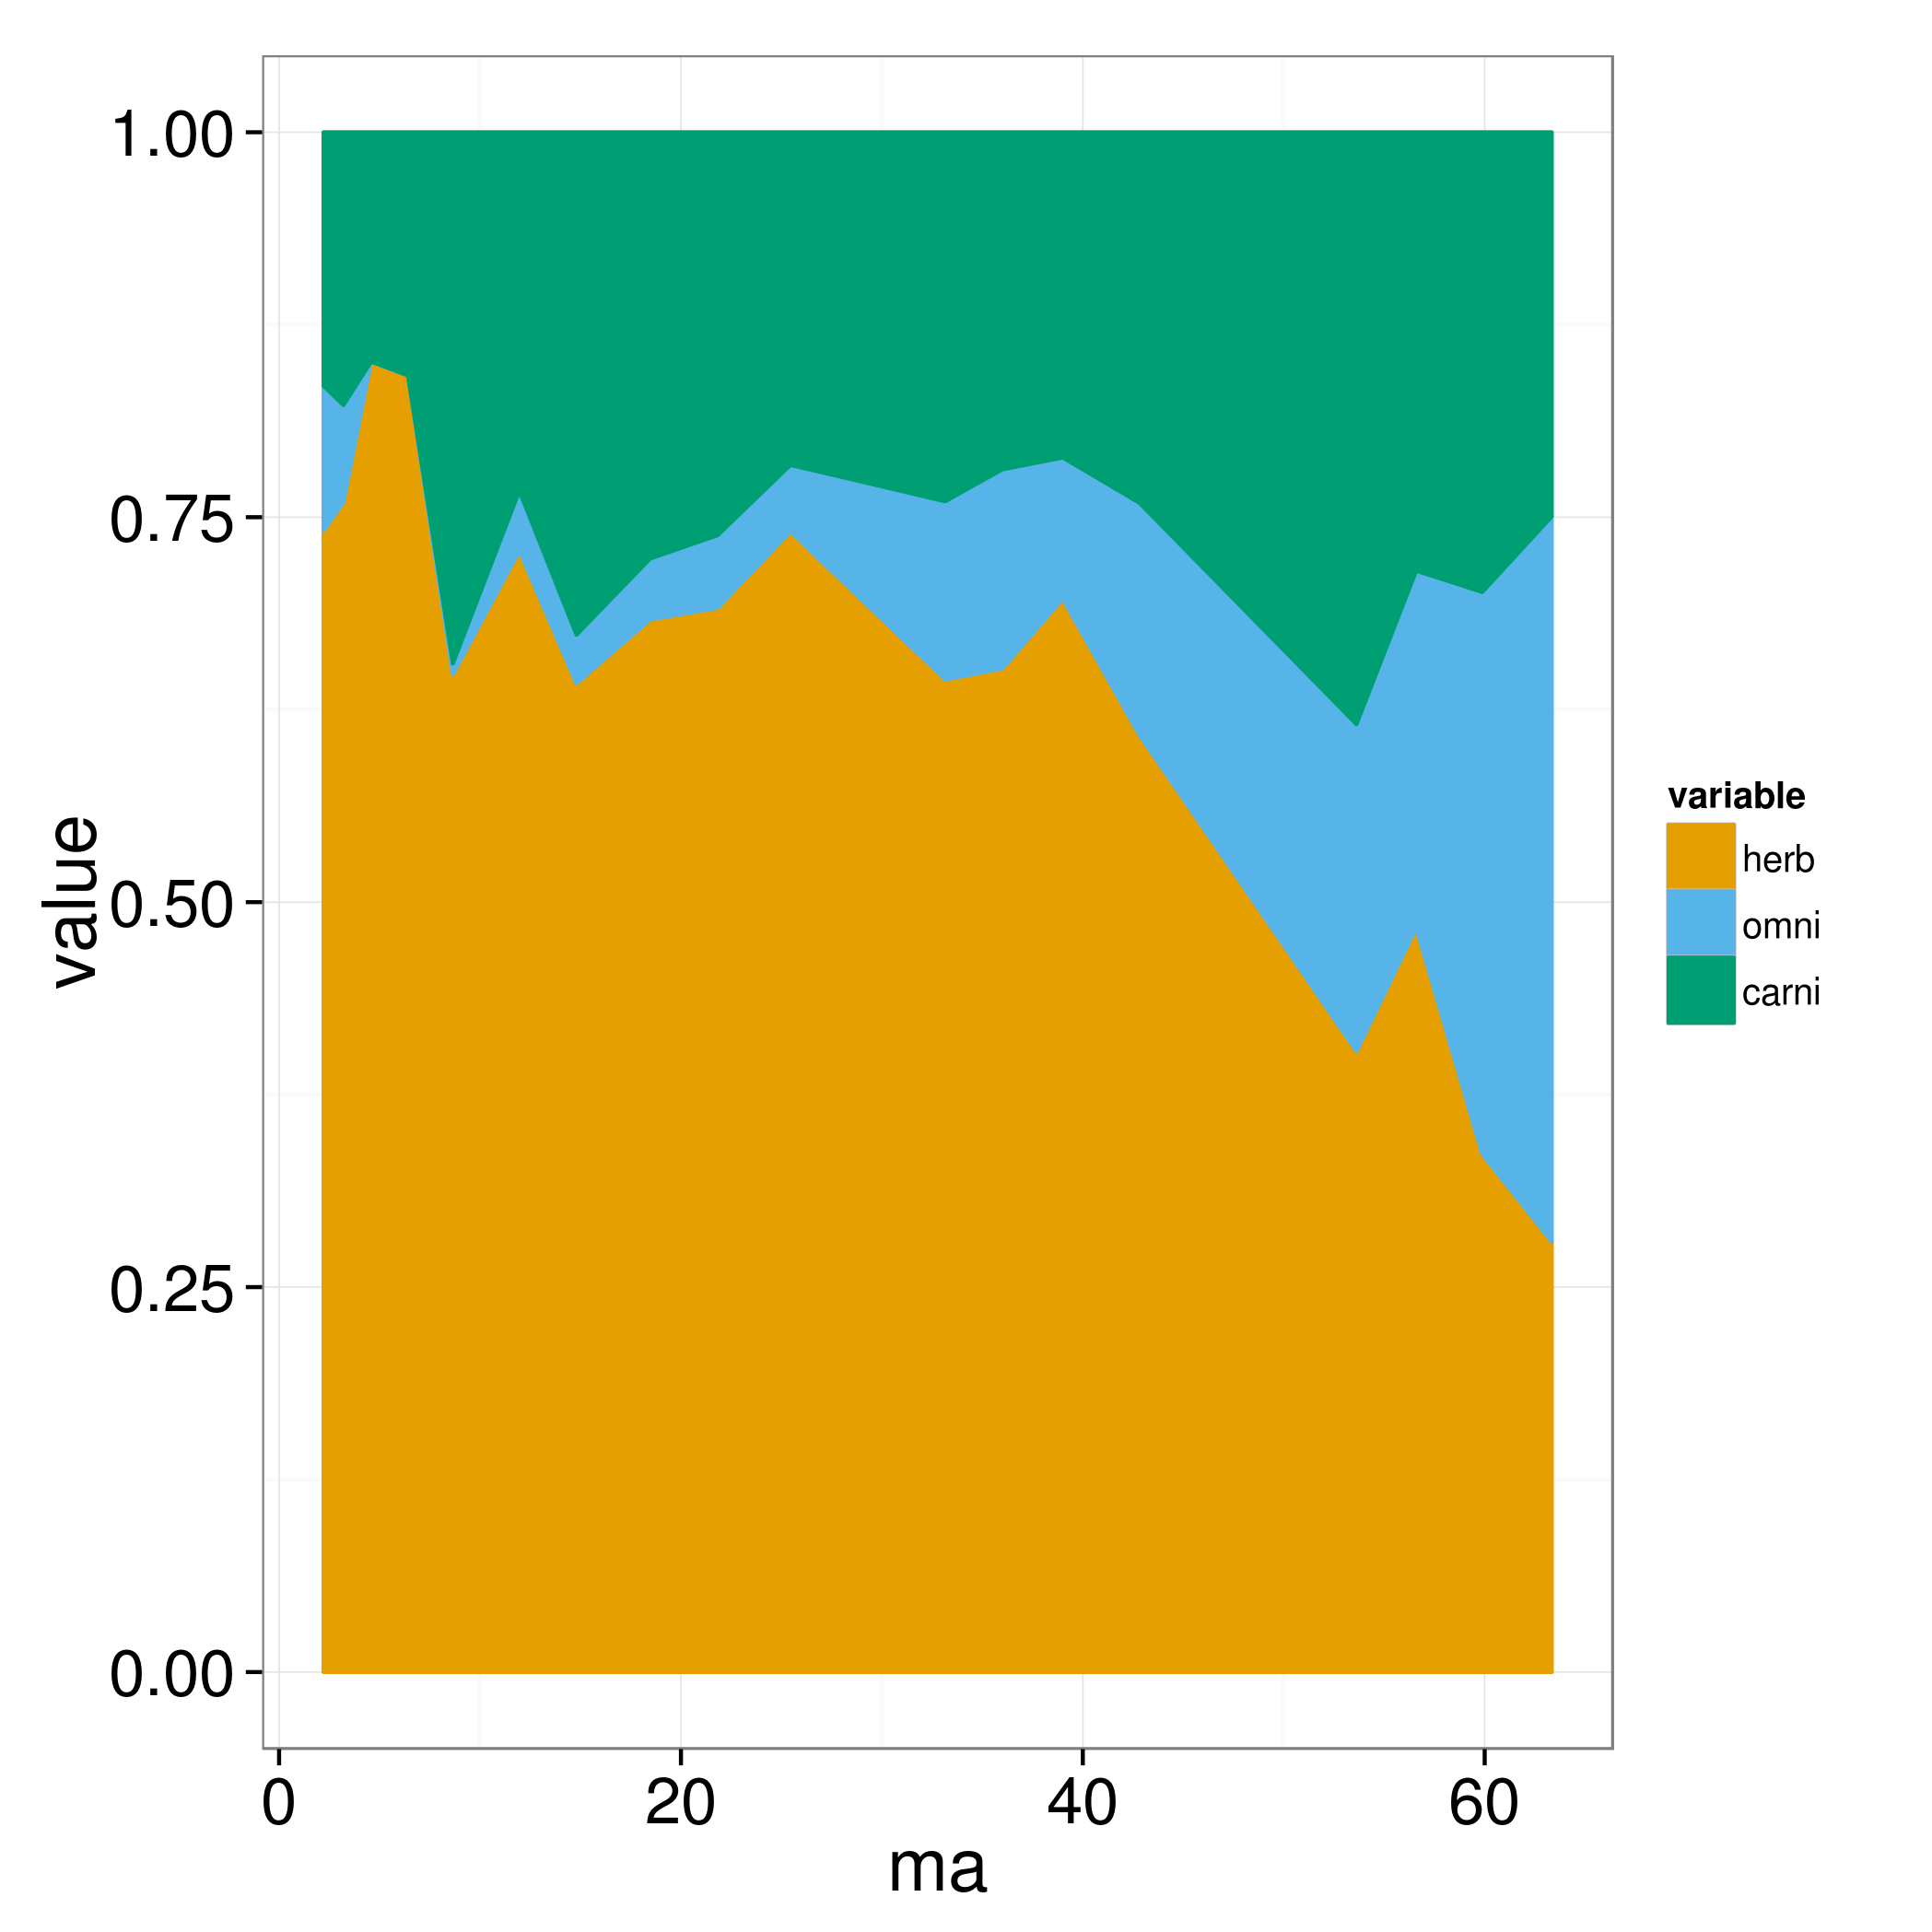
\includegraphics[width = \onecolwid]{figure/rel_diet}
        %  \end{center}
        %  \caption{Relative abundance of mammalian dietary categories.}
        %  \label{fig:rel_diet}
        %\end{figure}
      \end{block}
    \end{column}

    \begin{column}{\twocolwid}
      \begin{columns}[t,totalwidth = \twocolwid]
        \begin{column}{\onecolwid}
          \begin{block}{Results}

          \end{block}
        \end{column}

        \begin{column}{\onecolwid}
          \begin{block}{Fancy}
          \end{block}
        \end{column}
      \end{columns}

      \begin{alertblock}{Biogeographic networks}
        \begin{figure}[ht]
          \begin{center}
            \begin{subfigure}[b]{\onecolwid}
              \centering
              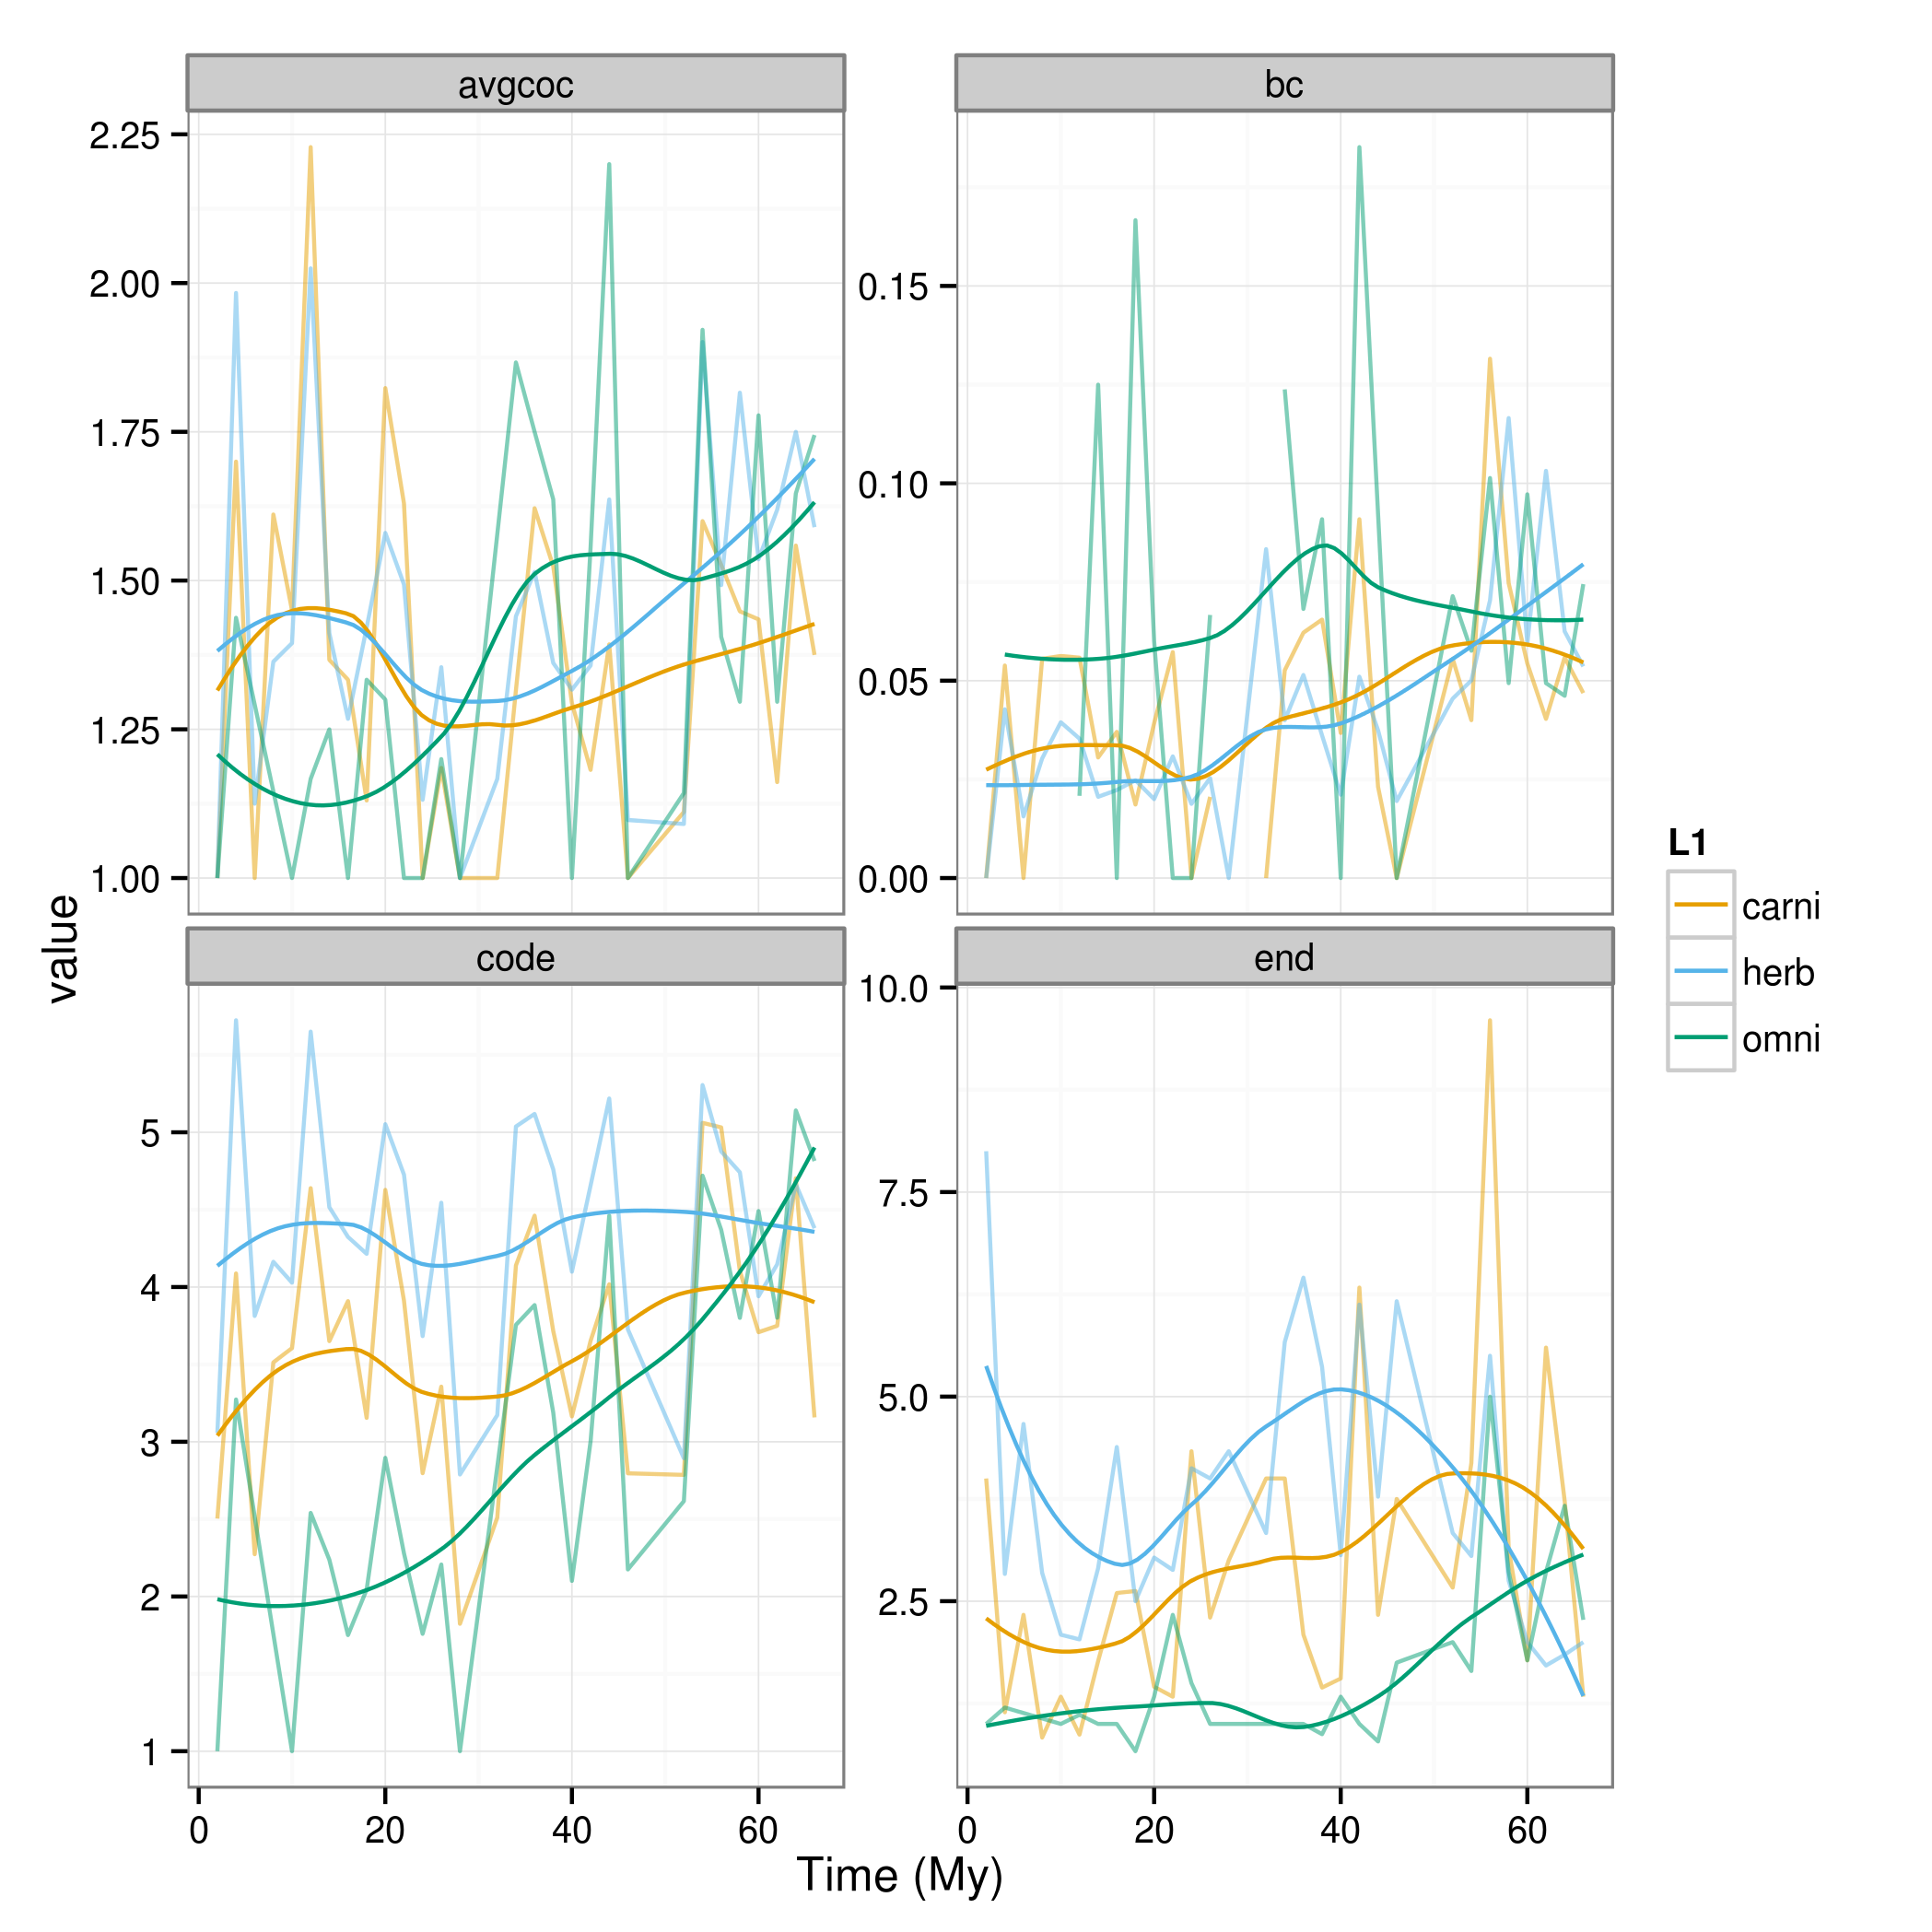
\includegraphics[width = \onecolwid]{figure/diet_bin}
              \label{fig:net_diet}
            \end{subfigure}
            \begin{subfigure}[b]{\onecolwid}
              \centering
              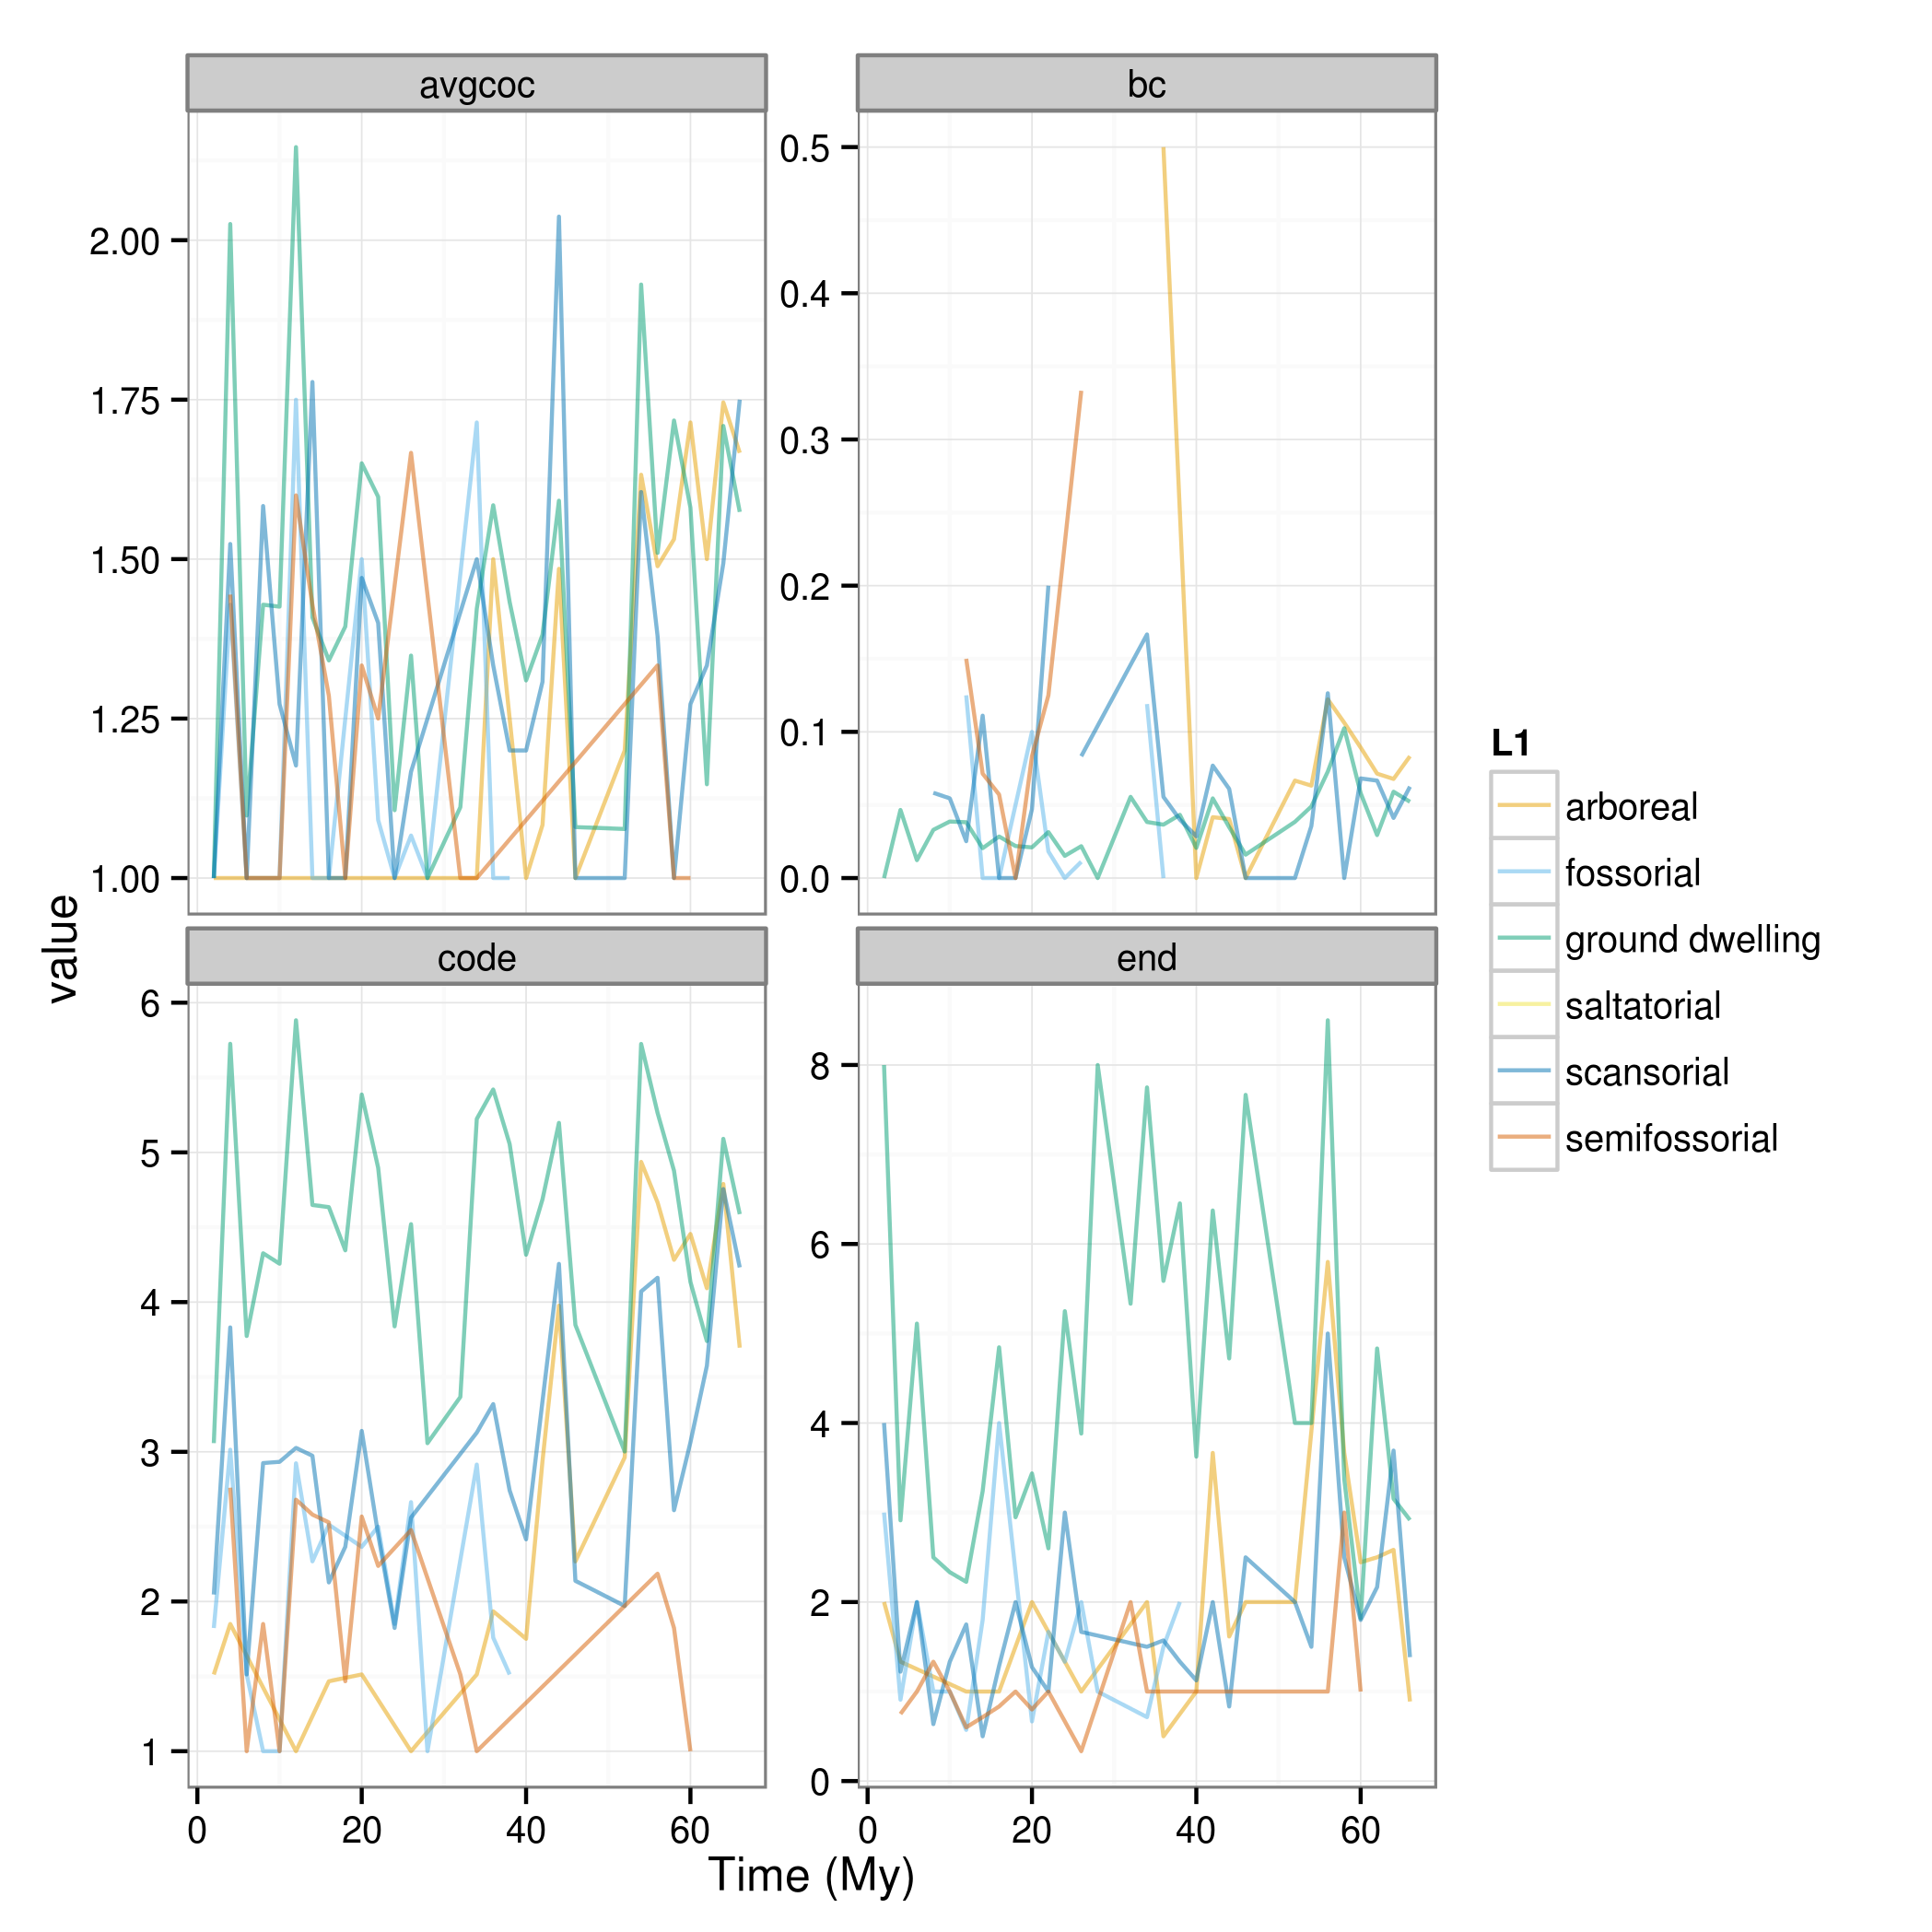
\includegraphics[width = \onecolwid]{figure/loco_bin}
              \label{fig:net_loco}
            \end{subfigure}
          \end{center}
          \caption{Biogeographic network summary statistics from the 2 My bins.}
          \label{fig:net_sum}
        \end{figure}
      \end{alertblock}

      \begin{columns}[t,totalwidth = \twocolwid]
        \begin{column}{\onecolwid}
          \begin{block}{Discussion}

          \end{block}
        \end{column}

        \begin{column}{\onecolwid}
          \begin{block}{Conclusions}
           
          \end{block}

          \begin{block}{Acknowledgements}
            John Alroy, Michael Foote, Ken Angielczyk.
          \end{block}

          % bibliography
          \begin{scriptsize}
            \begin{block}{Bibliography}
              \bibliographystyle{abbrvnat}
              \bibliography{cosmo_prov,packages}
            \end{block}
          \end{scriptsize}
        \end{column}
      \end{columns}
    \end{column}
  \end{columns}
\end{frame}
\end{document}
